%
% $Id$
%
% This describes the new design for the DODS server. It is based on
% a SDD template for software that has already been implemented but
% needs significant redesign and implementation. 7/21/2000 jhrg

\documentclass{article}
\usepackage{epsfig}
\usepackage{rotating}
% \usepackage{subfigure}
\usepackage{vcode}
\usepackage{xspace}
\usepackage{gloss}

% Change paragraph typesetting; eliminate indenting and add more space between
% paragraphs. 2/15/2000 jhrg
\setlength{\parindent}{0em}     % Amount of indentation
\addtolength{\parskip}{1ex}     % Vertical separation

% Note: to get the gloosary to work, run bibtex in the registry.gls.aux file,
% then latex registry, then bibtex *.gls, then latex. Also, make sure to set
% your BST and BIBINPUTS environment variables so that the BST and BIB files
% will be found.
\makegloss

% Sample macros including a URL which can be hyphenated. 
\newcommand{\httpd}{\texttt{httpd}\xspace}
\newcommand{\Cpp}{\rm {\small C}\raise.5ex\hbox{\footnotesize ++}\xspace}
\newcommand{\dap}{\rm {\small DAP}\raise.5ex\hbox{\footnotesize ++}\xspace}
\newcommand{\maewesturl}{http://maewest.gso.uri.edu/\-cgi-bin/\-nph-dsp/\-htn\_sst\_decloud/\-1992/\-i92098065016.htn\_d.Z\xspace}

\begin{document}

\title{DODS Server Changes}
\author{James Gallagher\thanks{The University of Rhode Island,
    jgallagher@gso.uri.edu}}
\date{\today \\ $Revision$ }

\bibliographystyle{plain}

\maketitle
\tableofcontents

\section{Introduction}

This document describes the current design and implemention of the DODS
servers and ways in which both the design and implementation should be
changed. The current design and its implementation are the result of several
years worth of accumlated ideas, their implementations and changes to
accomodate unforeseen situations. The result is an implementation that can be
significantly improved on a number of fronts with only modest effort. The
changes described here should be done incrementally so that the benefits of
each will be immediately available.

The reader is assumed to be familiar with DODS~\cite{DODS:home-page} and the
DODS User's Guide~\cite{DODS:users-guide}.

Section~\ref{sec:overview} provides an introduction along with a brief
rationale for each of the proposed changes.

Section~\ref{sec:arch} describes the current architecture of the DODS
servers. The focus here is on the current implementation.

Section~\ref{sec:design} describes a new design for a DODS server. This
design can be built incrementally using the existing server design combined
with new modules for new server responses.

Section~\ref{sec:new-features} describes new features for the DODS server.
There s considerable overlap between Sections~\ref{sec:design}
and~\ref{sec:new-features} since some of the new design changes depend on the
new features.

\section{Overview of the Proposed Changes}
\label{sec:overview}

DODS provides access to a number of different types of data sources using
servers. These servers are implemented as HTTP CGI programs. The network
management component of a DODS server is supplied by \httpd. The
server software specific to DODS is composed of seven discrete programs; a
dispatch program and six other programs which generate the server's different
responses to queries. 

The \Cpp implementations of the DODS servers provides access to six different
types of data sources.\footnote{The different data ources are: NetCDF, HDF,
  DSP and Matlab data files, JGOFS data system servers and files that can be
  read using the FreeForm package.} However, each type of data source has its
own dispatch script. To access a netCDF and an HDF file on the same machine,
two fundementally different DODS URLs \onlygloss{dods-url} must be used. More
importantly, users must remember to use the correct dispatch program for a
given data source type. This makes the servers more difficult to use because
people must know which types data sources are on each machine and, for those,
which dispatch program to name in the DODS URL. The collection of different
dispatch programs should be replaced with a single program.

In the current implementation, the six response generators (or handlers)
share a significant amount of software. The common functions of these
handlers are already segregated in a library (the \dap library, see the DODS
Programmer's Guide~\cite{DODS:prog-guide}. One change proposed in this
paper is to change the separate handlers' implementation so that they are all
libraries themselves containing only the software unique to their function.
The functions of what are now six seprarate programs can then be built into a
single executable image. Of course, this will save space but more importantly
it will streamline the server's maintenance.

DODS servers can become more efficient if the number of Unix \texttt{fork}
and \texttt{exec} operations can be reduced. In most cases CGI
programs\footnote{They are often called CGI scripts, but that's just because
  most early CGIs were implmented in Perl, as part of our servers are.
  There's no reason a CGI \emph{has} to be a script.} are started by a web
daemon\footnote{In this paper, I'm going to assume that web daemon in the
  Apache daemon and I'm going to call it \httpd. In practice, DODS
  servers run just fine under other daemons so long as they support CGI~1.1
  and HTTP~1.0.} and on Unix this usually entails both a \texttt{fork} and an
\texttt{exec}. These operations are expensive since both necessitate a change
from Unix's user-mode to kernel-mode. If the logic contained in the dispatch
program can be separated to a library, then the functions now contained in
the seven programs which currently comprise a DODS server can, in theory, be
implemented as a single exectuable. Doing so will cut down the number of
expensive OS operations from four (two \texttt{fork}s and two \texttt{exec}s)
to two.\footnote{The remaining \texttt{fork} and \texttt{exec} \emph{can} be
    avoided by using a daemon which runs CGIs in a thread, by making the
    DODS servers daemons in their own right or by using the Apache daemon's
    module system. As of 7/24/2000 a group at UCAR has done the later of
    these and is working on integrating their changes with the URI DODS
    software. It will be in the project's best interests to have \emph{both}
    types of servers since they represent two different ends of the
    performance versus complexity tradeoff.}
  
  The DODS servers currently make heavy use of Perl. While this has been an
  asset in the past because it provided us with a way to rapidly change our
  servers to meet new needs, there is a tradeoff in performance and features.
  Perl must first compile a script before executing it. Thus, accessing a
  DODS server 100 times translates into 100 invokations of Perl, each of
  which must first compile the dispatch program before executing it. That is
  the performance tradeoff. The feature tradeoff is that developers must be
  very careful of how they take advantage of Perl's flexibility. In addition,
  there are potential security problems with Perl scripts that are simpler to
  avoid with a standalone executable.\footnote{It \emph{is} possible to write
    secure Perl CGIs, but it takes some doing and future modifications can
    introduce new holes unless they are added carefully. The same can be said
    for CGIs written in \Cpp, but I think the problems are on a different
    order.} It is very easy to create a CGI using Perl which provides ways to
  circumvent the normal accounting and authentication schemes of a computer
  (i.e., they can be easy to hack).  Because DODS servers are more mature and
  less likely to need to change quickly, the functions now handled by Perl
  scripts should be r\"eimplemented in \Cpp.

\section{Current Architecture}
\label{sec:arch}

The description of the DODS servers in this section is brief. The focus of
this paper is on changes to the current design and implementation but it is 
hard to discuss those without some background in the current design. 

DODS servers are implemented using an off-the-shelf HTTP daemon. While there
are several different web daemons availale for UNIX, all of the known \Cpp
DODS servers are using either the Apache~\cite{apache:httpd} or the NCSA
daemon (both are called \httpd), on which the Apache deamon is based. The
DODS-specific parts of a DODS server are implemented as a CGI which is
started by \httpd. The CGI reads data from a data source and, based
on the URL used to invoke it, generates a reponse.

Figures~\ref{fig:dods-server} and~\ref{fig:current-deployment} show the
idealized and actual deployment of the server. In many cases the actual
deployment is such that the there are $N$ discrete servers for $N$ different
types of data sources, even though about 80\% of the software in any of the
servers is common to them all.

\begin{figure}[h]
\begin{center}
\epsfig{file=dods-server.eps,width=2.5in}
\caption{The DODS server architecture. DODS servers all implement the DAP 3.1
  interface, use a third-party web (HTTP) daemon and read data from an
  external data source. The design in this paper describes changes in the
  design so that one server can read from many types of data sources.}
\label{fig:dods-server}
\end{center}
\end{figure}

\begin{figure}
\begin{center}
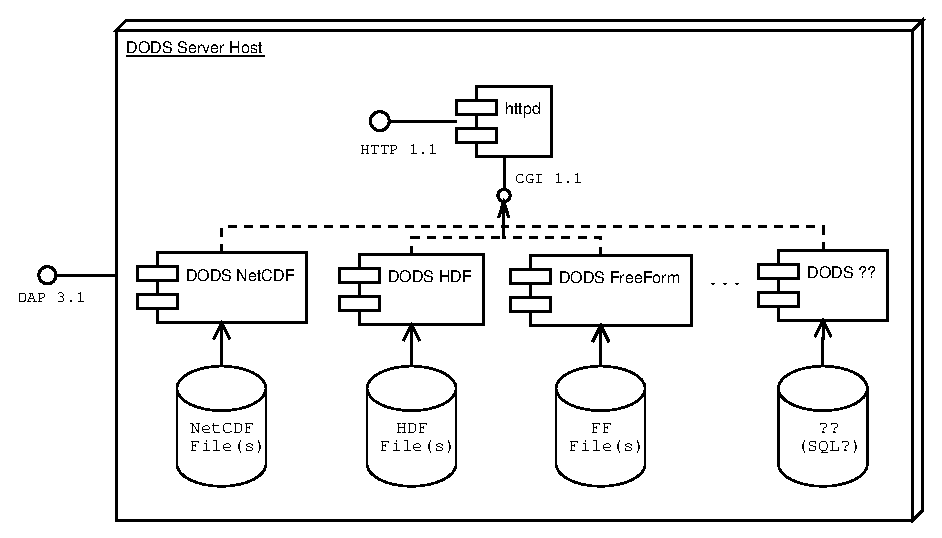
\epsfig{file=current-deployment.eps,width=4.5in}
\caption{A separate DODS server must be installed for each different type of
  data source. This makes it hard to define operations which can be applied to
  all of the data sources available from a single machine as well as
  complicting maintenance of the servers.}
\label{fig:current-deployment}
\end{center}
\end{figure}

\subsection{How URLs describe requests}

Given information about a DODS server's installation and the web pathname
\onlygloss{web-pathname} of a data source (typically a file, although that
does not have to be the case), it is fairly easy to derive the DODS URL for
that data source. 

Figure~\ref{fig:httpd-directories} shows the layout of three of the important
features of an \httpd installation. The \texttt{DocumentRoot} directory holds
the pathnames to the data sources. In the figure, the document root
subdirectories named \texttt{data/nc}, \texttt{data/hdf} and \texttt{data/ff}
are there for example only; any valid Unix file or directory names can be
used.  The \texttt{ScriptAlias} directory is used by \httpd to hold CGI
programs.  The \texttt{ServerRoot} directory holds configuraton files used by
the daemon.  For example, suppose that in the \texttt{data/nc} directory
there is a data file named \texttt{fnoc1.nc} and that the DODS server
dispatch CGI is named \texttt{nph-nc}.  For completeness, suppose that the
domain name of the host running the server configured as shown in
Figure~\ref{fig:httpd-directories} is \texttt{dcz.dods.org}. The DODS URL for
this dataset would be
\begin{equation}
\texttt{http://dcz.dods.org/cgi-bin/nph-nc/data/nc/fnoc1.nc}
\label{url:simple}
\end{equation}
URL~\ref{url:simple} will return an error when typed into a web
browser\footnote{NB: This URL \emph{will} work when passed to a DODS client
  program but that's because those programs know they are dealing with a DODS
  URL and know how to append the various suffixes to get different responses.
  A web browser known nothing about DODS so the user must append the
  suffix.}, however, because the server has not been asked to return any
result. Thus, the server returns a response which explains that the request
was an error, why and how to form a valid request.

A DODS server can return three different type of objects unique to DODS and
four responses that can be used by many different programs including web
browsers. Each of the different responses is requested by appending a suffix
to the $<path>$ component of the DODS URL. The suffixes and the response they
generate are:
\begin{description}
\item[.das] Return the DODS DAS object, encoded as ASCII text.
\item[.dds] Return the DODS DDS object, encoded as ASCII text.
\item[.dods] Return the DODS DataDDS object, encoded in a multipart MIME
  document. 
\item[.asc] Return data in a CSV format which can be read by spreadsheet
  programs.
\item[.html] Return an HTML form which automatically builds a constraint
  expression that describes which data in the data source to access.
\item[.info] Return an HTML document which combines the metadata and
  ancillary data stored with the data source in a way that is easy(ier) to
  read than the text representation of the DAS and DDS objects.
\item[/] This suffix is unlike all the others in that it is added to the
  end of a directory name, \emph{not} a data source name. When the $<path>$
  part of a DODS URL ends in a slash (\texttt{/}) the server returns a
  listing of the named directory.
\end{description}
Thus to request HTML encoded metadata about the FNOC dataset shown in
URL~\ref{url:simple} you would append the suffix \texttt{.info} to the URL

\begin{equation}
\texttt{http://dcz.dods.org/cgi-bin/nph-nc/data/nc/fnoc1.nc.info}
\label{url:info}
\end{equation}

Accessing data from a DODS server usually involves more than simply appending
the suffix \texttt{.dods} or \texttt{.asc} to a URL. That is because most of
the time a data source holds far more information than the user (either human
or computer) wants or needs. DODS uses constraint expressions
\onlygloss{constraint} to describe the parts of a data source that are
desired. For example, suppose a particular data file contains five variables,
but a user wants only two of those variables. A constraint expression can be
used to request that only those two variables be included in the server's
response to the request for data. A constraint expression is supplied using
the Query String \onlygloss{query-string} part of a URL. Even though the
syntax of the constraint expression language is fairly simple, describing it
is outside the scope of this paper. The syntax is fully described in the DODS
User's Guide~\cite{DODS:users-guide}. However, here are two example URLs with
constraints
\begin{equation}
\texttt{http://dcz.dods.org/cgi-bin/nph-nc/data/nc/fnoc1.nc.dods?u,v}
\label{url:ce1}
\end{equation}
\begin{equation}
\texttt{http://dcz.dods.org/} \cdots \texttt{/fnoc1.nc.dods?u[0:5][0][0:2:10]}
\label{url:ce2}
\end{equation}
URL~\ref{url:ce1} requests that data contained in just the variables $u$ and
$v$ be included in the response. URL~\ref{url:ce2} stipulates that only $u$
be returned and further limits the parts of the three dimensional
array\footnote{How did I know it was a three dimensional array? Look at the
  output of the DDS or Info responses from the server.} to the first six
rows, only column $0$ and the six planes numbered $0, 2, 4, \cdots, 10$.

\begin{figure}[h]
\begin{center}
\epsfig{file=httpd-directories.eps,width=4.5in}
\caption{A typical directory structure for an Apache \texttt{httpd}
  installation (this is the installation found on RedHat Linux; other Unix
  installations might use different directories, but the essential
  organization is the same). Note that the directories \texttt{data/nc},
  \texttt{data/hdf} and \texttt{data/ff} are examples. The actual collection
  of directories, their names and contents have no more restrictions than any
  other directory on a Unix computer.}
\label{fig:httpd-directories}
\end{center}
\end{figure}

\subsection{Components of the server}
The component labeled \emph{DODS Access} in Figure~\ref{fig:dods-server} is
actually made up of a collection of components, each implemented as either a
Perl script or as a \Cpp executable image.
Figure~\ref{fig:current-deployment} shows the components of the DODS Access
component. The following sections describes each of these components.

\subsubsection{CGI dispatch}
\subsubsection{DAS handler}
\subsubsection{DDS handler}
\subsubsection{Data handler}
\subsubsection{Info handler}
\subsubsection{HTML handler}
\subsubsection{ASCII handler}

\begin{figure}[h]
\begin{center}
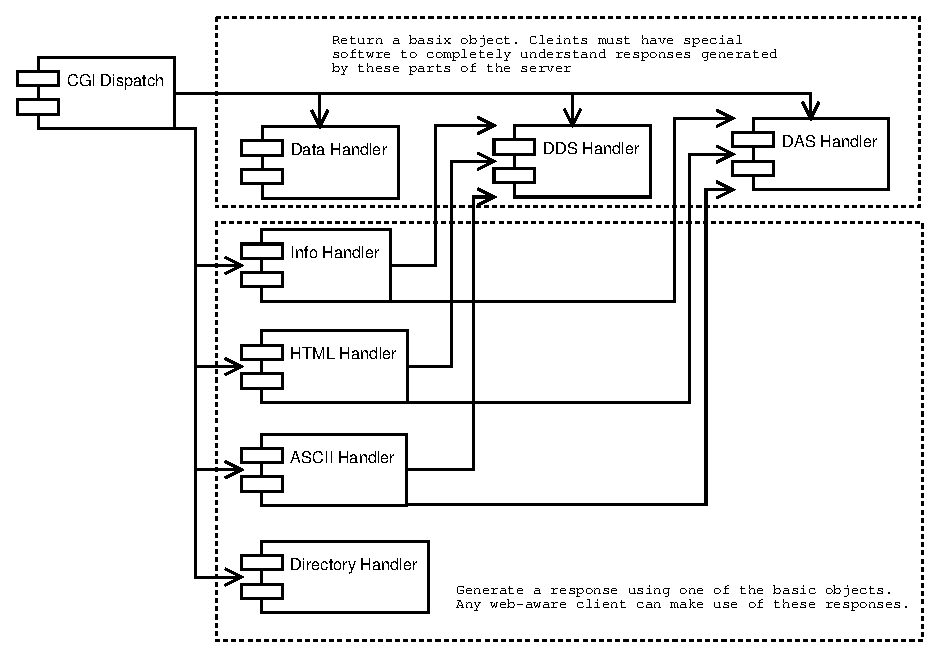
\epsfig{file=current-server-arch.eps,width=4.25in}
\caption{The sub-components of a DODS Access component. The DODS Access
  component in Figure~\ref{fig:dods-server} is actually and aggregation of
  several components, each of which is currently a separate executable.}
\label{fig:current-server-arch}
\end{center}
\end{figure}

\section{Changes in Design and Implementation}
\label{sec:design}

\subsection{Combine the dispatch scripts}
The first change to make to the DODS servers implementation is to re-design
the dispatch scripts so that a single script can be used by all of the
servers. This change in the interface to the DODS servers provides the basis
for a number of other changes to DODS so it should be done before the other
changes described in this paper. 

Working from the example server configuration in
Figure~\ref{fig:httpd-directories} and the URL numbers~\ref{url:simple}
through~\ref{url:ce2}, let there are two additional files available on
the server, each one of a different type. Suppose those files' pathnames are
data/hdf/2000415.HDF and data/ff/1998-6-avhrr.dat. Using the current
multi-dispatch scheme the three data sources would be accessed by 
\begin{equation}
\texttt{http://dcz.dods.org/cgi-bin/nph-nc/tdata/fnoc1.nc}
\label{url:old1}
\end{equation}

\begin{equation}
\texttt{http://dcz.dods.org/cgi-bin/nph-hdf/tdata/2000415.HDF}
\label{url:old2}
\end{equation}

\begin{equation}
\texttt{http://dcz.dods.org/cgi-bin/nph-ff/tdata/1998-6-avhrr.dat}
\label{url:old3}
\end{equation}

Using a single dispatch script makes only the URLs' $<path>$ component unique
for a given host. The URLs~\ref{url:old1}, \ref{url:old2} and~\ref{url:old3}
become 
\begin{equation}
\texttt{http://dcz.dods.org/cgi-bin/nph-dods/tdata/fnoc1.nc}
\label{url:new1}
\end{equation}

\begin{equation}
\texttt{http://dcz.dods.org/cgi-bin/nph-dods/tdata/2000415.HDF}
\label{url:new2}
\end{equation}

\begin{equation}
\texttt{http://dcz.dods.org/cgi-bin/nph-dods/tdata/1998-6-avhrr.dat}
\label{url:new3}
\end{equation}

This change will effectively fix a design flaw in the directory service
feature of the DODS servers. See Section~\ref{sec:directory}.

The new script will be slightly more complex than any of the existing scripts
since it must distinguish between the different data sources and their
corresponding DAS, DDS and DataDDS handlers. To do this the new dispatch
script can use the server configuration file described in
Section~\ref{sec:config}. 

\subsection{A single executable}
This change will simplify installation and maintenance and provide a way to
combine the CGI-based server with the daemon-based server developed at UCAR.

\subsection{Improvements to the HTML handler}
The HTML handler will provide a way for users to get HDF, netCDF, Matlab and
IDL files containing the data requested by users. See
Section~\ref{sec:add-resp}.

\subsection{Improvements to the directory listing response}
\label{sec:directory}
There are a number of bugs which need to be fixed; some of these stem from
the current implementation, that is based heavily on Perl. The directory
service can be significantly improved over the long term by rewriting it in
\Cpp.

By taking the different dispatch scripts and coalescing them into a single
script, the major flaw with the directory service will be fixed. That is,
that as users navigate a directory hierarchy they will get errors when
clicking on files or data sources whose types don't match the type of server
they named in the URL.

\section{New Features for the DODS Server}
\label{sec:new-features}

\subsection{Add a configuration file}
\label{sec:config}
This will make explicit a number of features/characteristics of the DODS
server(s) that are now implicitly encoded using the interactions of the
servers' various components. The configuration file will use regular
expressions to map file/data-sources to a particular type of handler. 

\subsection{Additional responses}
\label{sec:add-resp}
The design of each of the new file-format handlers can be based on the design
of the \texttt{asciival} handler. Of the four formats we will support, netCDF
directly supports almost all of the DODS datatypes and it has a simple \Cpp
API, so it should be the simplest to implement. The other formats will
require extra work because some DODS data types don't map into their API and
must be recast to other types before the file can be written.

The four file types for which handlers must be written are:
\begin{itemize}
\item netCDF
\item HDF
\item Matlab
\item IDL
\end{itemize}

Each of the file types has an API library which can be used to create the
file and write it contents.

Figures~\ref{fig:file-format-main}, \ref{fig:file-format-types1} and
\ref{fig:file-format-with-attrs} show one way to build a handler for the
file-type output. Each of the figures uses the netCDF handler as an example.

In Figure~\ref{fig:file-format-main} the format handler for netCDF is shown
as a class named ncwriter. The ncwriter program could be implemented either
as a class which is instantiated by \texttt{main} or it can be \texttt{main}
itself.  Either way, it contains instances of Connect, DDS, DataDDS, and in a
later version, DAS and MetatdataProcessing.

In ncwriter, an instance of Connect is used to access the DDS and DataDDS
(and later DAS) of a dataset referenced by a DODS URL. The returned objects
are used to access each variable requested by the DODS URL.

The \dap library defines classes which holds values of byte, integer, \ldots,
variables as well as container types such as Structure which can be used to
group collections of variables. Aggregate types in DODS are similar to
\texttt{struct}s in C. Note in Figure~\ref{fig:file-format-types1} that these
datatype classes (e.g., Byte) are abstract and that they inherit from the
abstract class BaseType. Since the classes are abstract, they must be
subsclassed, and their abstract methods realized, to be instantiated. In this
design, those subclasses are named NCWriterByte, \textit{et cetera}.

Each of the concrete datatype classes (e.g., NCWriterByte) inherits from the
\emph{interface} NCWriter. NCWriter is an abstract class that contains the
method \texttt{write\_variable}. Each of the concrete datatype classes must
realize this method. 

The \texttt{write\_variable} method will be used to add a particular type of
variable to an open netCDF file. The ncwriter program can do some thing like
the following:

\begin{vcode}

DataDDS datadds;
.
.
.
NcFile nc(path, NcFile::Replace);

for (Pix p = datadds.first_var(); p; datadds.next_var(p)) {
    NCWriter *ncw = dynamic_cast<NCWriter *>(datadds.var(p));
    ncw->write_variable(nc);
}

\end{vcode}

Note that the sniplet of code does not show reading the DataDDS from the
remote dataset\footnote{Look at the asciival program in
  \texttt{DODS/src/tools/asciival} for examples of reading DAS, DDS and
  DataDDS objects.} but that must be done before variables in the DataDDS can
be used. Since the DODS datatypes have been subclassed, the object referenced
by the BaseType pointer returned by DDS::var(Pix) must be an instance of the
subclasses (i.e., it must be an instance of one of the concrete classes
NCWriterByte, \ldots, NCWriterGrid) and thus we must also be able to cast
them to the abstract class NCWriter. Once cast to a NCWriter pointer, we can
use the write\_variable method contained in the concrete class (without
having to figure out which exact class is referenced by the BaseType
pointer).

For both the HDF and netCDF file format handlers it will be necessary to
include attribute information about each variable in the generated file. This
can be added once the basic handler is working.
Figure~\ref{fig:file-format-with-attrs} shows one possible deign that can be
used to simplify matching a variable's value with its attribute table
object.\footnote{The DAS object contains a set of AttrTable objects, one for
  each variable in the dataset plus others which contain `global' attributes
  (attributes which apply to the entire dataset).}

Writing attribute information for each variable will be simplified if their
attributes are copied from the DAS object (which stores attributes for all
the variables) into each variable. If that is done, then each variable will
be able to write its attribute information without first looking it up in the
DAS.  The MetadataProcessing class transfers the attribute information to the
variable's internal attribute table object (called AttrTable in
Figure~\ref{fig:file-format-with-attrs}) by moving each variable's attributes
from the DAS.

An attribute table is added to each of the concrete datatype objects in much
the same way that the \texttt{write\_variable} method was added; by defining
an abstract class which provides and interface to the AttrTable object.
However, in this case, each of the concrete datatype classes must also
contain an instance of AttrTable. The attribute tables can then be accessed
by casting instances of the concrete datatypes to
AttributeInterface.\footnote{This design has already been realized by the
  Matlab command line client. Look at the source code in
  \texttt{DODS/src/clients/ml-cmdln}. In particular, look at the write\_val
  source files.}

\begin{figure}[h]
\begin{center}
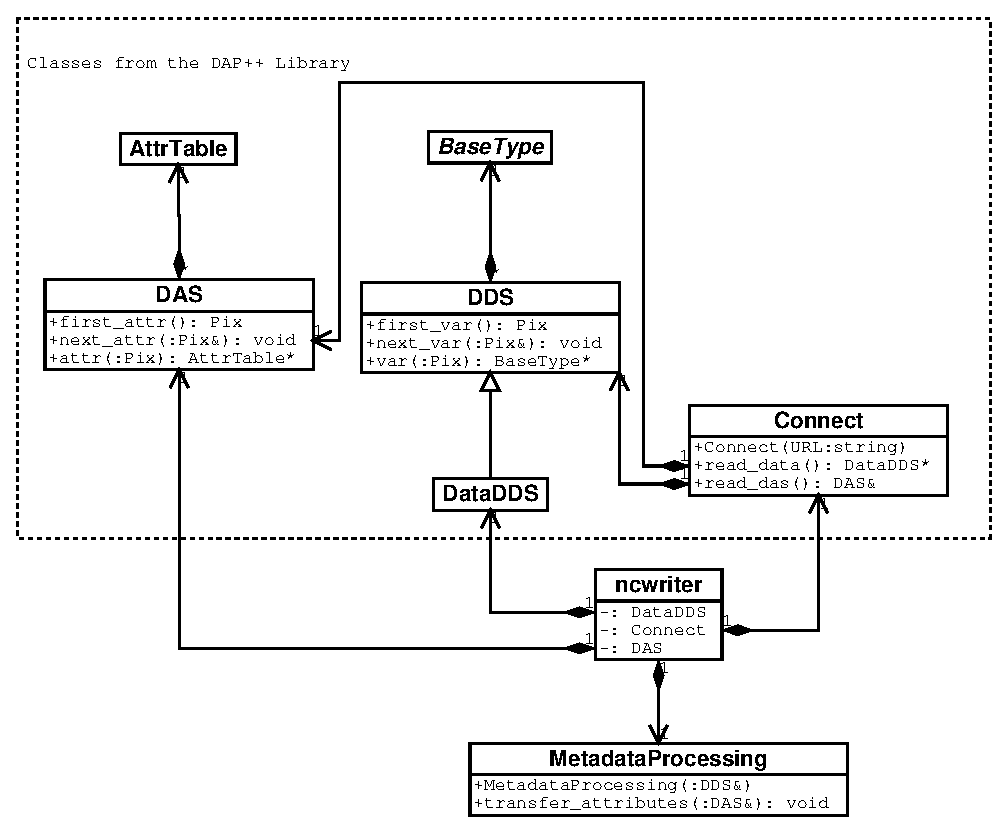
\epsfig{file=file-format-writer2.eps,width=4.25in}
\caption{The program ncwriter (represented here as a class) is a simple DODS
  client that uses the Connect class to access the DDS (and in the future the
  DAS). Methods in those classes are used to access parts of the dataset.
  Note that the MetadataProcessing and DAS classes are used to add
  `attributes' to the variables. HDF and netCDF support attributes while
  Matlab and IDL do not. For the Matlab and IDL file-format handlers this
  should be ignored. See also Figure~\ref{fig:file-format-with-attrs}.}
\label{fig:file-format-main}
\end{center}
\end{figure}

\begin{sidewaysfigure}[h]
\begin{center}
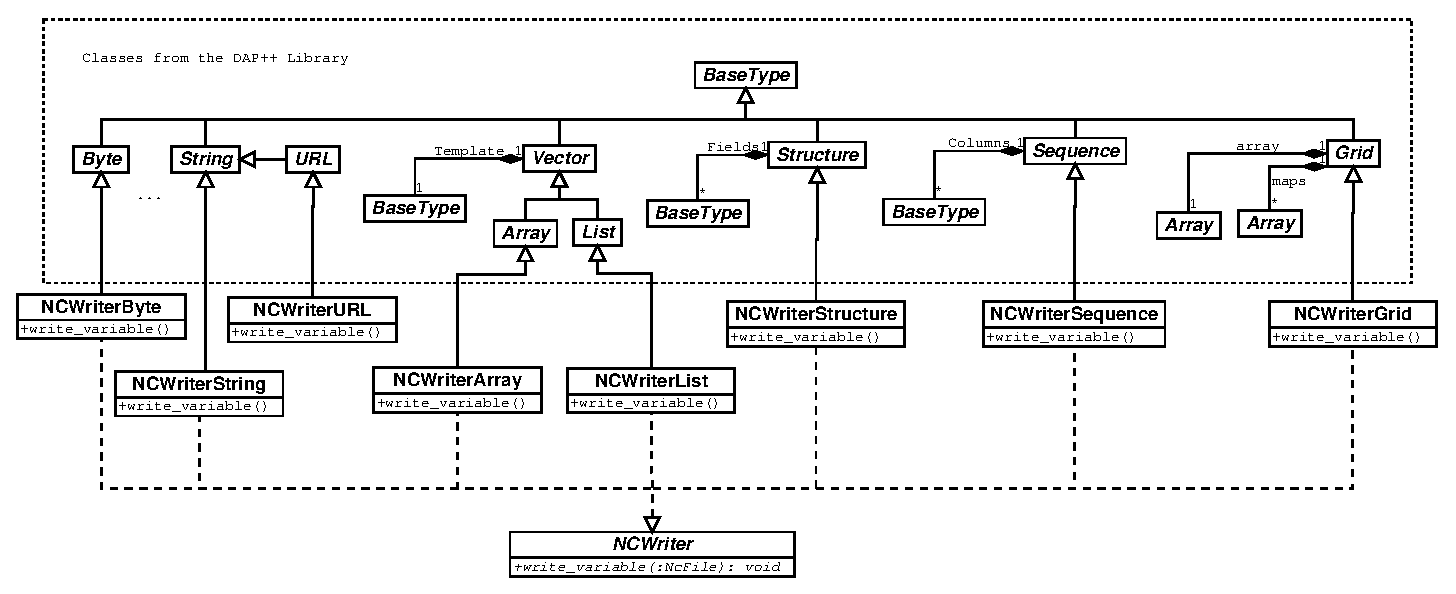
\epsfig{file=file-format-writer.eps,width=8.25in}
\caption{Subclassing the \dap library's datatype hierarchy provides a way to
  write out variables. Even though the \texttt{print\_val} method was
  designed for printing ASCII representations of the variables, it can be used
  to write binary values, too}
\label{fig:file-format-types1}
\end{center}
\end{sidewaysfigure}

\begin{sidewaysfigure}[h]
\begin{center}
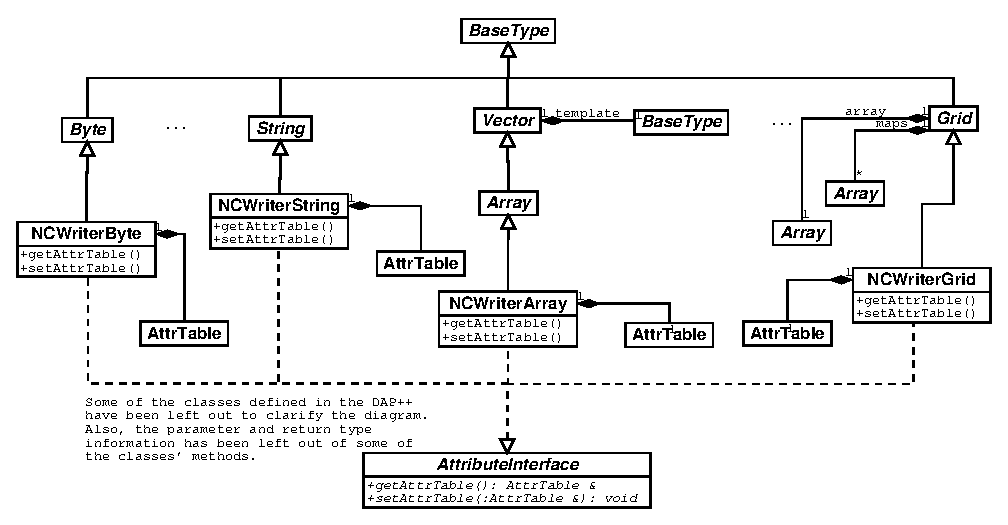
\epsfig{file=file-format-with-attrs.eps,width=8.25in}
\caption{Adding attribute processing capabilities to the datatype classes.}
\label{fig:file-format-with-attrs}
\end{center}
\end{sidewaysfigure}

\subsection{An HTML home page}

\clearpage
\appendix

\section{ChangeLog}
\begin{verbatim}

$Log: dods-server-sdd.tex,v $
Revision 1.6  2000/10/25 16:35:16  jimg
Changed the design of the file-format handlers.

Revision 1.5  2000/08/23 21:34:12  jimg
Added diagrams and a brief explanation of the file format handlers.

Revision 1.4  2000/08/06 05:23:41  jimg
Rev of 8/4/2000

Revision 1.3  2000/07/27 18:05:22  jimg
Added text describing most of the current design and implementation of the
servers. I have not added text for each of the C++ executables, but will
later, depending on what needs to be explained.
Added a skimpy outline for the Changes.

Revision 1.2  2000/07/25 21:49:46  jimg
Added text for the overview section. Added a glossary.

Revision 1.1  2000/07/21 16:49:08  jimg
Started. Added three figures for the current state of affairs.

\end{verbatim}

\printgloss{dods-glossary}

\raggedright

\bibliography{dods}

\end{document}
